% Chapter 4
\chapter{Lizard and Its Implementation}
\label{ch:lizard}

\section{Lizard attention}
\label{sec:lizard-attn}

Lizard~\cite{lizard} replaces every softmax attention layer of the teacher with two branches (\cref{fig:lizard-layer}). The teacher projections $W_Q$, $W_K$, $W_V$ and $W_O$ stay as they are. Lizard adds five small parameters to each layer.

\begin{description}[leftmargin=0.6cm,style=nextline]
\item[Gated branch] Gated linear attention (\cref{eq:gla}) with Hedgehog feature maps $\phi_q$ and $\phi_k$ (\cref{eq:hedgehog}). The gate is one scalar for each token, $\gamma_i = \sigma(W_\gamma \vx_i)$. All 32 heads of a layer share the feature maps and the gate. The branch divides by its own row sum, so its weights sum to 1.
\item[Window branch] Softmax attention over the last $w = 128$ keys, with $m = 4$ sink logits in the denominator (\cref{eq:window}). The paper calls it \emph{anchor window attention}. It has no RoPE.
\item[Output] The two branches add up: $\hat\vy_i = \hat\vy^{\text{gate}}_i + \alpha\, \hat\vy^{\text{win}}_i$, with one learnable $\alpha$ for each layer.
\end{description}

\begin{figure}[t]
\centering
\resizebox{\linewidth}{!}{%
\begin{tikzpicture}[
  font=\small, >={Stealth[length=2.2mm]}, node distance=6mm,
  box/.style={draw=#1, fill=#1!10, rounded corners=1.5pt, align=center, inner sep=4pt, line width=0.6pt},
  teacher/.style={box=teachercolor, text width=3.4cm},
  lizard/.style={box=lizardcolor, text width=3.9cm},
  small/.style={box=lizardcolor, text width=1.6cm},
  opt/.style={draw=changecolor, fill=changecolor!8, dashed, rounded corners=1.5pt, align=center, inner sep=4pt, text width=3.9cm, line width=0.6pt},
  arr/.style={->, draw=inksecondary, line width=0.6pt}]
\node[box=teachercolor, text width=1.6cm] (x) at (0,0) {input $\vx_i$};
\node[teacher] (proj) at (0,-1.35) {$W_Q,\ W_K,\ W_V$\\ \footnotesize teacher weights};
\node[small, text width=1.7cm] (gate) at (-6.8,-3.0) {gate $W_\gamma$\\[1pt] \footnotesize $\sigma(W_\gamma \vx_i)$};
\node[lizard] (phi) at (-3.6,-3.0) {Hedgehog maps $\phi_q,\ \phi_k$\\ \footnotesize shared by the 32 heads};
\node[opt] (rope) at (3.6,-3.0) {RoPE on $\vq,\ \vk$\\ \footnotesize only in \code{window_rope}};
\node[lizard] (gla) at (-3.6,-4.85) {\textbf{Gated branch}\\ \footnotesize all keys $t \le i$, weight $\prod_{l=t+1}^{i}\gamma_l$, own row sum};
\node[lizard] (win) at (3.6,-4.85) {\textbf{Window branch}\\ \footnotesize softmax over the last 128 keys};
\node[small] (sink) at (6.6,-4.85) {sinks\\ $t_1, \dots, t_4$};
\node[circle, draw=lizardcolor, fill=lizardcolor!10, inner sep=1.5pt, line width=0.6pt] (alpha) at (3.6,-6.35) {$\times\,\alpha$};
\node[circle, draw=inksecondary, inner sep=1pt, line width=0.6pt] (plus) at (0,-7.05) {$+$};
\node[teacher] (oproj) at (0,-8.1) {$W_O$\\ \footnotesize teacher weight};
\node[box=teachercolor, text width=1.6cm] (y) at (0,-9.25) {output};
\draw[arr] (x) -- (proj);
\draw[arr] (x.west) -| (gate.north);
\draw[arr] (proj.south) -- ++(0,-0.4) -| (phi.north);
\draw[arr] (proj.south) -- ++(0,-0.4) -| (rope.north);
\draw[arr] (phi) -- (gla);
\draw[arr] (rope) -- (win);
\draw[arr] (gate.south) |- node[pos=0.75, above, font=\footnotesize, text=inksecondary] {$\gamma_i$} (gla.west);
\draw[arr] (sink) -- (win);
\draw[arr] (proj.south) -- node[right, font=\footnotesize, text=inksecondary, pos=0.6] {$\vv$} (0,-4.85) -- (gla.east);
\draw[arr] (0,-4.85) -- (win.west);
\draw[arr] (win) -- (alpha);
\draw[arr] (alpha) |- (plus);
\draw[arr] (gla) |- (plus);
\draw[arr] (plus) -- (oproj);
\draw[arr] (oproj) -- (y);
\node[box=lizardcolor, minimum width=4mm, minimum height=3mm, inner sep=0pt] (l1) at (-6.4,-8.65) {};
\node[right=1mm of l1, font=\footnotesize, align=left] {Lizard parameters,\\trained in stage 1};
\node[box=teachercolor, minimum width=4mm, minimum height=3mm, inner sep=0pt] (l2) at (-6.4,-9.45) {};
\node[right=1mm of l2, font=\footnotesize, align=left] {teacher weights,\\LoRA in stage 2};
\end{tikzpicture}%
}
\caption[One Lizard attention layer]{One Lizard attention layer. The teacher projections give the queries $\vq$, the keys $\vk$ and the values $\vv$. Blue parts are the Lizard parameters. Gray parts are the weights of the teacher. The purple RoPE box is the change of \cref{ch:rope}. The original Lizard has no RoPE in either branch.}
\label{fig:lizard-layer}
\end{figure}

\Cref{tab:lizard-params} lists the parameters of one layer. Lizard adds 18,437 parameters to each layer and 294,992 to the 16 layers. This is 0.024\% of the model.

\begin{table}[ht]
\centering
\small
\caption[The Lizard parameters of one layer]{The Lizard parameters of one layer, with feature dimension 128 (project notes, document~1).}
\label{tab:lizard-params}
\begin{tabularx}{\linewidth}{@{}llrL@{}}
\toprule
Parameter & Shape & Count & Function \\
\midrule
\code{phi_q}, \code{phi_k} & $64 \times 128$ each & 16,384 & Feature maps with 256 features. All heads share them. \\
\code{W_gamma} & $2048 \times 1$ & 2,048 & Gate. Start value 0, so $\gamma = 0.5$ at the start. \\
\code{meta_tokens} & 4 & 4 & Sink logits in the window denominator \\
\code{alpha_blend} & 1 & 1 & Weight $\alpha$ of the window branch. Start value 1. \\
\midrule
Total & & 18,437 & \\
\bottomrule
\end{tabularx}
\end{table}

\section{The two training stages}
\label{sec:stages}

\Cref{fig:stages} shows the two stages as the paper describes them.

\textbf{Stage 1: attention transfer.} Only the Lizard parameters train. Each Lizard layer gets the input of the teacher layer. The teacher computes its own output with RoPE. The loss compares the two outputs of each layer:
\begin{equation}
\mathcal{L}_{\text{MSE}} = \frac{1}{N} \sum_{l=1}^{N} \left\| \mathbf{Y}^{l}_{\text{softmax}} - \hat{\mathbf{Y}}^{l}_{\text{Lizard}} \right\|_F^2 .
\label{eq:stage1}
\end{equation}
The code of this work uses 1000 times the mean squared error of each layer. This form differs from \cref{eq:stage1} only by a constant factor, and the Adam optimizer does not change with such a factor.

\textbf{Stage 2: fine-tuning.} LoRA weights on the attention projections train with the next-token loss. In the code of this work, the Lizard parameters stay frozen in stage 2. The paper does not say if they train.

\begin{figure}[t]
\centering
\begin{subfigure}{0.82\linewidth}
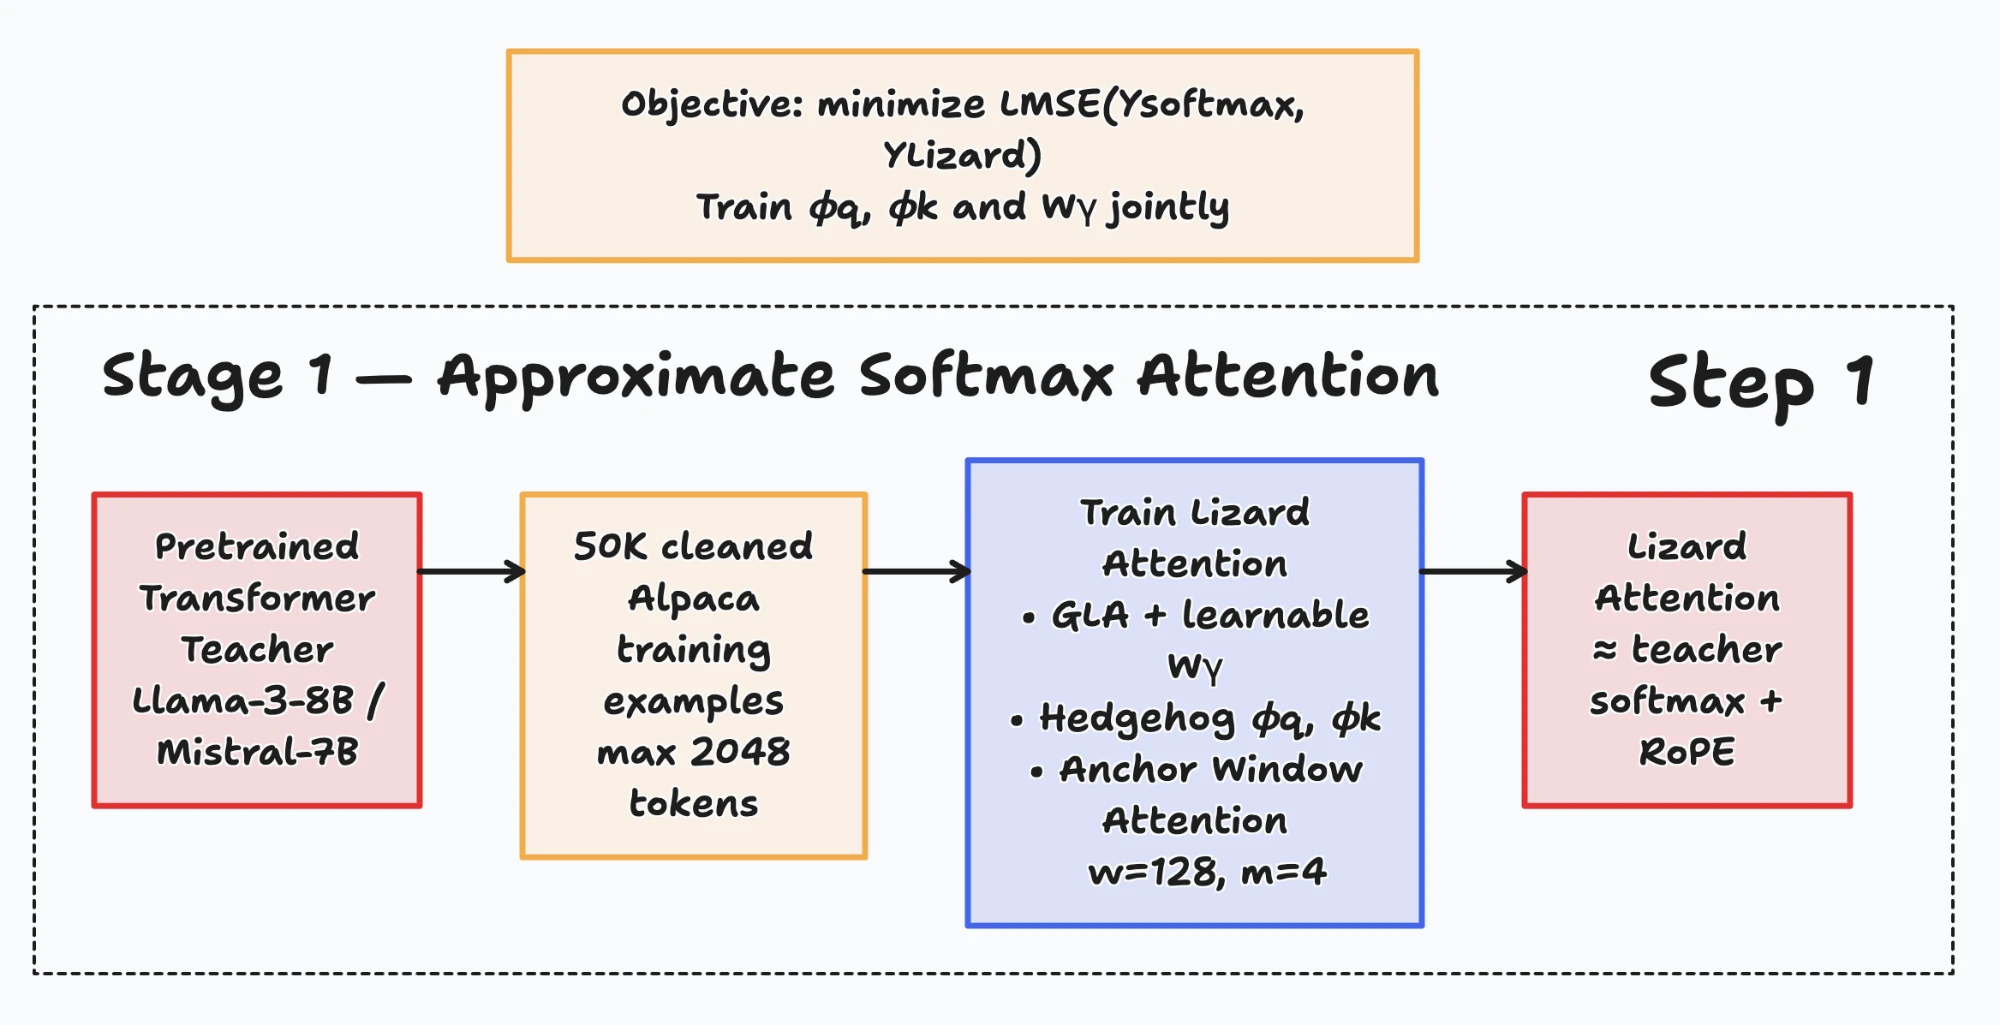
\includegraphics[width=\linewidth]{lizard-stage1}
\caption{Stage 1: attention transfer with the MSE loss.}
\end{subfigure}\\[6pt]
\begin{subfigure}{0.82\linewidth}
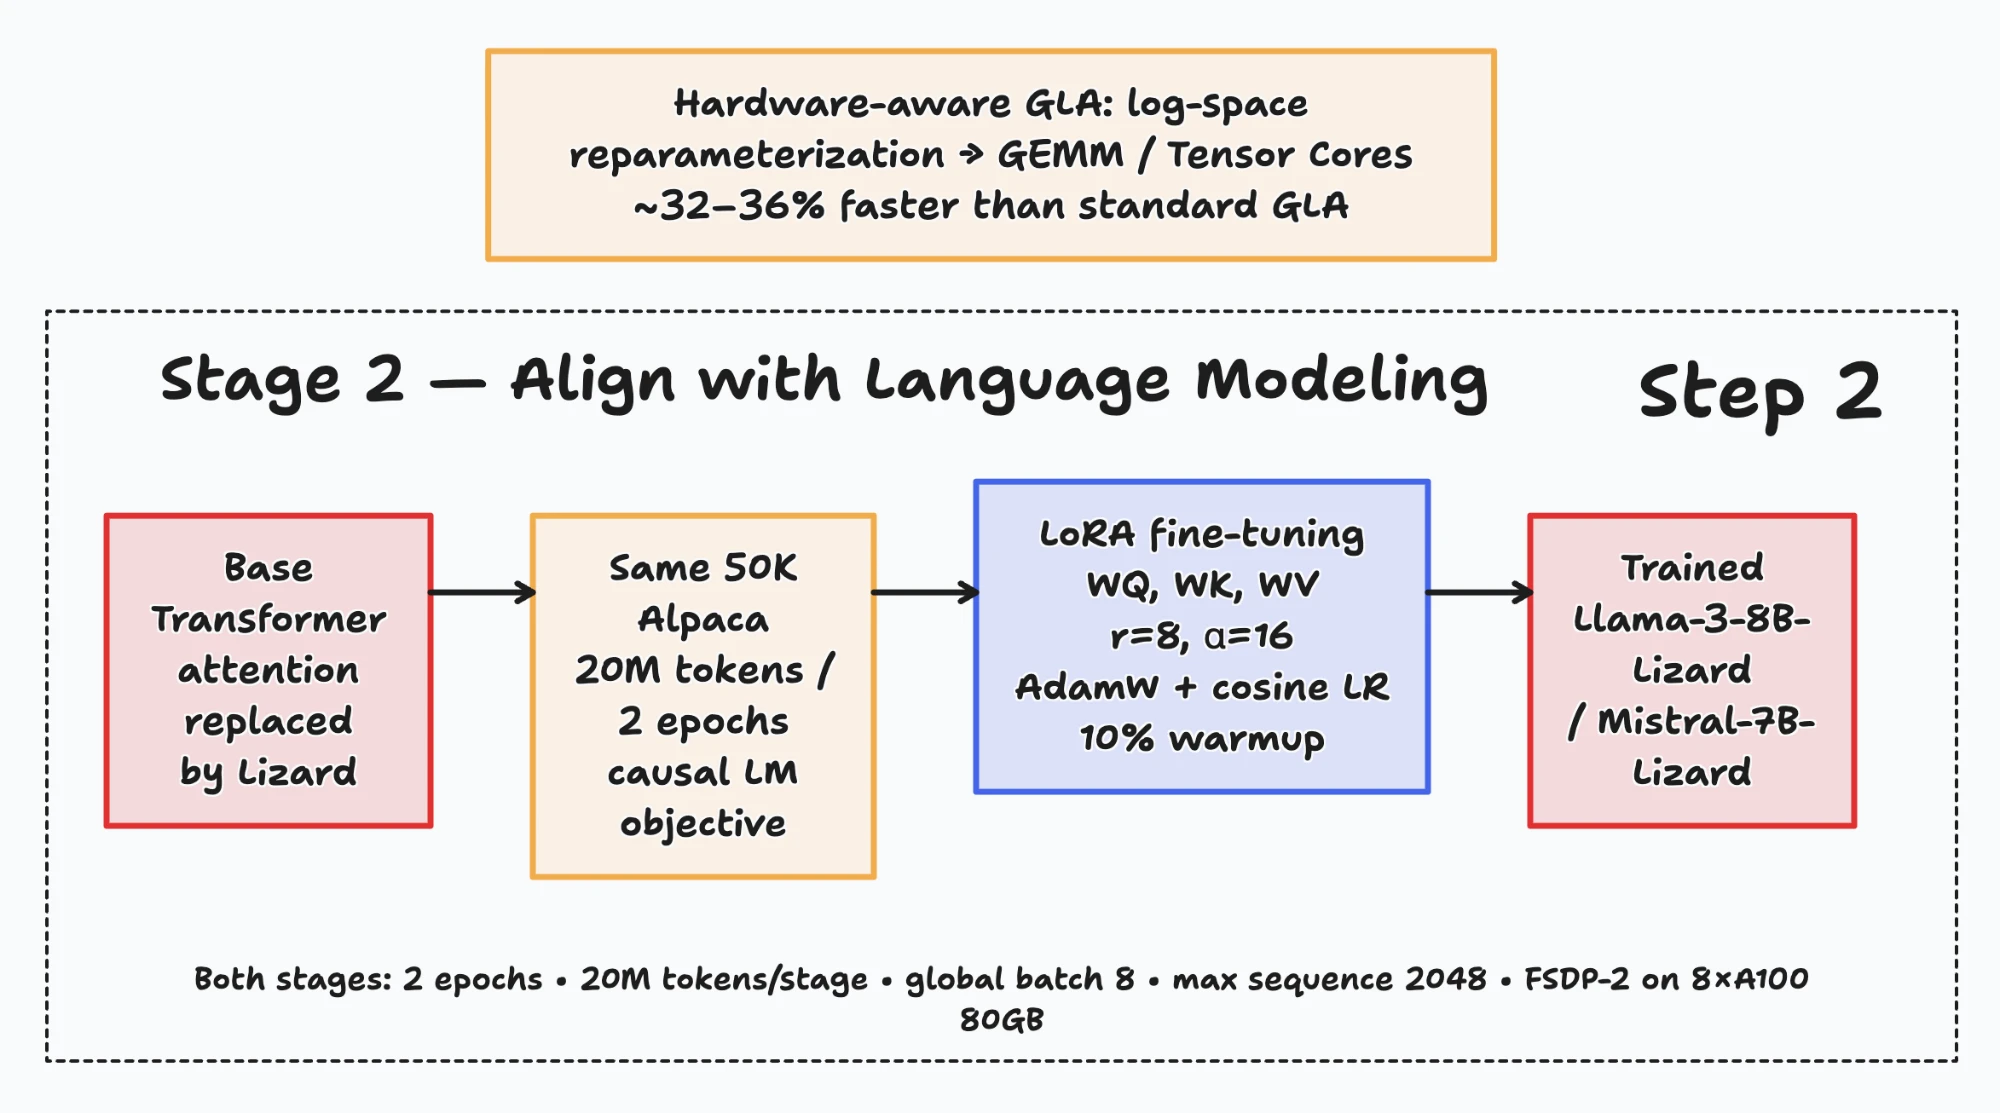
\includegraphics[width=\linewidth]{lizard-stage2}
\caption{Stage 2: LoRA with the next-token loss.}
\end{subfigure}
\caption[The two training stages of Lizard]{The two training stages of Lizard, as the paper describes them. The paper uses 8B teachers in this description. This thesis uses Llama-3.2-1B. Source: the figures of the project notes, drawn by the author.}
\label{fig:stages}
\end{figure}

\section{The training algorithm in log space}
\label{sec:logspace}

Section~4 of the paper gives a fast algorithm for the gated branch. In matrix form, the branch needs the cumulative gate products $c_t = \prod_{j \le t} \gamma_j$ and the quotients $c_i / c_t$. The products get very small, and bf16 cannot store them. The paper moves $\log c_t$ into the exponent of the feature maps, so that the branch becomes one matrix product.

A proof audit of this work found a limit (\cref{tab:proofs}, P3). The step holds for the exponential feature map. With the softmax feature map of Table~13, the term $\log c_t$ cancels in the softmax, and the gate disappears. Also, $1/c_t$ overflows after approximately 126 tokens at $\gamma = 0.5$, so only a form that works in chunks can use it. This work does not use the fast algorithm. It computes the parallel form of \cref{eq:gla} in float32 and materializes the full $L \times L$ matrix.

\section{The reference implementation}
\label{sec:reference}

The work started with a reference implementation in the repository \code{jku-thesis}~\cite{jkurepo}. It is pure PyTorch. The functions \code{hedgehog}, \code{gla} and \code{awa} implement the formulas directly, and a class \code{LizardAttention} joins them. A second file contains slow loop and recurrent versions of every formula. These versions are the ground truth. The tests compare the two versions in float64 and require a relative error below $10^{-10}$. Further adapters compare the branches with external implementations, for example the GLA kernels of the \code{flash-linear-attention} library and PyTorch attention with a sink column.

\section{The port to LoLCATs}
\label{sec:port}

The training of this work uses the LoLCATs code base~\cite{lolcats,lolcatsrepo}. It already has the two stages, the data pipeline and the evaluation. The functions of the reference code went into LoLCATs without changes. A wrapper class connects them with the LoLCATs model:

\begin{itemize}
\item It takes the teacher attention module and uses its projections again. Thus only the five Lizard parameters are new.
\item In stage 1, it computes the teacher output with RoPE as the target. It returns the student output and the target to the trainer. The next layer gets the teacher output.
\item In evaluation and generation, it uses a cache. The cache keeps the state of the gated branch and the keys and values of the last 128 tokens. A prompt runs in one dense pass. Each new token then uses the recurrent form.
\end{itemize}

\Cref{tab:jku-vs-lolcats} shows the differences between the two code bases. The LoLCATs recipe became the first recipe of this work, because the task was to keep the existing configs.

\begin{table}[ht]
\centering
\small
\caption[The reference pipeline against the LoLCATs pipeline]{The reference pipeline (\code{jku-thesis}) against the LoLCATs pipeline of the first runs (project notes, document~1).}
\label{tab:jku-vs-lolcats}
\begin{tabularx}{\linewidth}{@{}lLL@{}}
\toprule
Aspect & Reference pipeline & LoLCATs pipeline \\
\midrule
Stage 1 loss & Summed squared error for each layer & 1000 $\times$ mean squared error for each layer \\
Stage 2 parameters & LoRA on $q, k, v$ and the Lizard parameters & LoRA on $q, k, v, o$. Lizard parameters frozen. \\
Precision & float32 & bf16 model, Lizard computations in float32 \\
Recipe & The recipe of the paper & The LoLCATs configs: learning rate $10^{-2}$ in stage 1 and $10^{-4}$ in stage 2 \\
\bottomrule
\end{tabularx}
\end{table}

\section{Tests of the attention layer}
\label{sec:tests}

The poor first results (\cref{ch:repro}) raised the question of a bug. Two levels of tests ran on CPU.

\textbf{Level 1: the formulas.} A small module made the 28 tests of the reference code run against the LoLCATs functions. 26 tests passed. The two other tests need a newer version of the \code{transformers} library and fail for the same reason on the reference code. The tests show these properties: the feature maps are positive, and each half sums to 1. The gated branch matches the loop form and the recurrent form. The window with sinks matches its loop form. Future tokens give no gradient. The gradients match finite differences.

\textbf{Level 2: the model.} A tiny Llama with random weights in float64 tested the wrapper, the conversion of the model and the cached paths. The output with the cache equals the dense output up to float64 rounding.

\begin{finding}
The tests show that the code computes the equations of the paper, and that the evaluation path computes the same function as the training path. They do not test the quality of the trained weights.
\end{finding}

\section{The paper against the code}
\label{sec:paper-vs-code}

A line-by-line comparison of the formulas of the paper with the code found 17 differences. Most of them have no effect. \Cref{tab:open-points} lists the points where the paper allows more than one reading.

\begin{table}[ht]
\centering
\small
\caption[Open points of the paper]{Open points of the paper and the choice of the code (project notes, documents~9, 13 and \enquote{math against code}).}
\label{tab:open-points}
\begin{tabularx}{\linewidth}{@{}>{\raggedright\arraybackslash}p{3.3cm}LL@{}}
\toprule
Point & What the paper says & Choice of the code \\
\midrule
D1: normalization of the gated branch & The parallel form has a denominator. The recurrent form and the matrix form have none. & Denominator (row sum 1) \\
D2: feature maps for each head & Not given. The LoLCATs default has one map for each head. & One map for all heads of a layer \\
D3: activation & Section 4 gives $\exp$. Table 13 gives softmax. & Softmax \\
D5: sink term & The equation has $\sum_j t_j$, but the text calls $t_j$ a logit. & $\sum_j \exp(t_j)$ \\
Gate start value & Not given & $W_\gamma = 0$, so $\gamma = 0.5$ \\
$\alpha$ & Not listed as a learnable parameter in the loss & Learnable, start value 1 \\
\bottomrule
\end{tabularx}
\end{table}

The written sink term $\sum_j t_j$ can make the denominator zero or negative (\cref{tab:proofs}, P4). Thus the code follows the word \enquote{logit}.

\section{Lizard attention v2: one option for each reading}
\label{sec:v2}

A second attention file (v2) makes each open point an option. With the default options, v2 gives exactly the outputs of v1. \Cref{tab:v2-options} lists the options.

\begin{table}[ht]
\centering
\small
\caption[The options of Lizard attention v2]{The options of Lizard attention v2. The first value is the default (project notes, document~13).}
\label{tab:v2-options}
\begin{tabularx}{\linewidth}{@{}lp{3.3cm}L@{}}
\toprule
Option & Values & Meaning \\
\midrule
\code{gla_norm} & \code{row}, \code{none}, \code{joint}, \code{hybrid} & Row sum of the gated branch (D1). \code{joint} and \code{hybrid} use one denominator for both branches and the sinks. \code{hybrid} is the LoLCATs form. \\
\code{alpha_per_head} & false, true & One $\alpha$ for each head \\
\code{alpha_init} & 1.0, any number & Start value of $\alpha$ \\
\code{feature_map_per_head} & false, true & One feature map for each head (D2) \\
\code{feature_activation} & softmax, exp & D3 \\
\code{gate_per_head} & false, true & One gate for each head \\
\code{gate_bias_init} & none, a number & A bias in the gate with a start value \\
\code{window_rope} & false, true & RoPE in the window branch only \\
\bottomrule
\end{tabularx}
\end{table}

\section{Proofs and float64 tests}
\label{sec:proofs}

The options depend on claims about the formulas. A proof audit checked each claim by hand. A float64 script then computed the smallest cases. \Cref{tab:proofs} lists the main claims.

\begin{table}[ht]
\centering
\small
\caption[Main claims of the proof audits]{Main claims of the proof audits (project notes, documents~13, 14 and 15). \enquote{Restricted} means: true only under the stated condition.}
\label{tab:proofs}
\begin{tabularx}{\linewidth}{@{}lLl@{}}
\toprule
Claim & Statement & Verdict \\
\midrule
P1 & The recurrent form equals the parallel form, without and with the denominator & Proved \\
P2 & The window share of a head is at most $\alpha / (1 + \alpha)$ & Restricted: $\alpha \ge 0$ \\
P3 & The log-space form equals the gated matrix form & Only for the $\exp$ map \\
P4 & The written sink term $\sum_j t_j$ can make the denominator 0 or negative & Proved \\
P5 & The decode forms of \code{joint} and \code{window_rope} equal their parallel forms & Proved \\
P6 & \code{joint} keeps a usable share for the gated branch at the start & Refuted \\
P7 (H) & Four sink logits with equal start values stay equal, so they act as one sink & Proved \\
P8 (C) & The total weight of a Lizard row is $1 + \alpha\rho_i$, more than 1 & Proved \\
P9 & With \code{hybrid} and $\gamma = 1$, the window share falls as $1/i$ & Restricted \\
P10 (F) & A window without RoPE cannot give exact previous-token attention in layer 0 & Restricted: no position input \\
\bottomrule
\end{tabularx}
\end{table}

Three claims matter most for the later chapters. P8 shows that a Lizard row is not a weighted mean of values: its weights sum to more than 1. P2 shows that $\alpha$ limits how much a head can take from the exact window. P10 shows that the window without RoPE cannot find the previous token from the positions.

\section{Lizard, LoLCATs, GLA and Liger in formulas}
\label{sec:fourmethods}

With the notation $\kappa_{it} = \phi(\vq_i)^\top\phi(\vk_t)$, the gate products $c_{it}$ and the window scores $s_{it}$, the outputs of Lizard and LoLCATs are
\begin{align}
\text{Lizard:}\quad \vy_i &= \frac{\sum_{t \le i} c_{it}\, \kappa_{it}\, \vv_t}{\sum_{t \le i} c_{it}\, \kappa_{it}} + \alpha\, \frac{\sum_{t \in W_i} e^{s_{it}} \vv_t}{\sum_{j} e^{t_j} + \sum_{t \in W_i} e^{s_{it}}}, \\
\text{LoLCATs:}\quad \vy_i &= \frac{\sum_{t \in W_i} a\, e^{s_{it}} \vv_t + \sum_{t \le i - w} \kappa_{it}\, \vv_t}{\sum_{t \in W_i} a\, e^{s_{it}} + \sum_{t \le i - w} \kappa_{it}} .
\end{align}
LoLCATs gives an exact weighted mean of the values. Its linear part excludes the window tokens. Lizard counts the window tokens twice, one time in each branch (claim B of document~15). The \code{hybrid} option of v2 equals LoLCATs under three conditions (claim A). All gates are 1, there are no sinks, and the linear sums cover only $t \le i - w$.

\section{Numerical stability: the NaN crash}
\label{sec:nan}

The first full run stopped in stage 2 at gradient step 386. The forward pass gave NaN, and a debugger breakpoint in the trainer then ended the job. A review found two operations without protection:

\begin{itemize}
\item The window branch computed $\exp(\vq^\top\vk/\sqrt{d})$ directly. In float32, $\exp$ overflows above approximately 88.7, and $\infty/\infty$ gives NaN. LoRA trains the query and key projections in stage 2, so the scores can grow.
\item The gated branch divides by the row sum. If all weights of a row underflow to 0, the result is $0/0$.
\end{itemize}

The fix subtracts the largest score and the largest sink logit before $\exp$, and it gives the row sum a small lower limit. Both changes keep the formulas the same. The overflow is the most probable cause, but no test reproduced it on the real checkpoint.
